

\begin{figure}[!htp]
\begin{center}
\begin{ccTexOnly}
  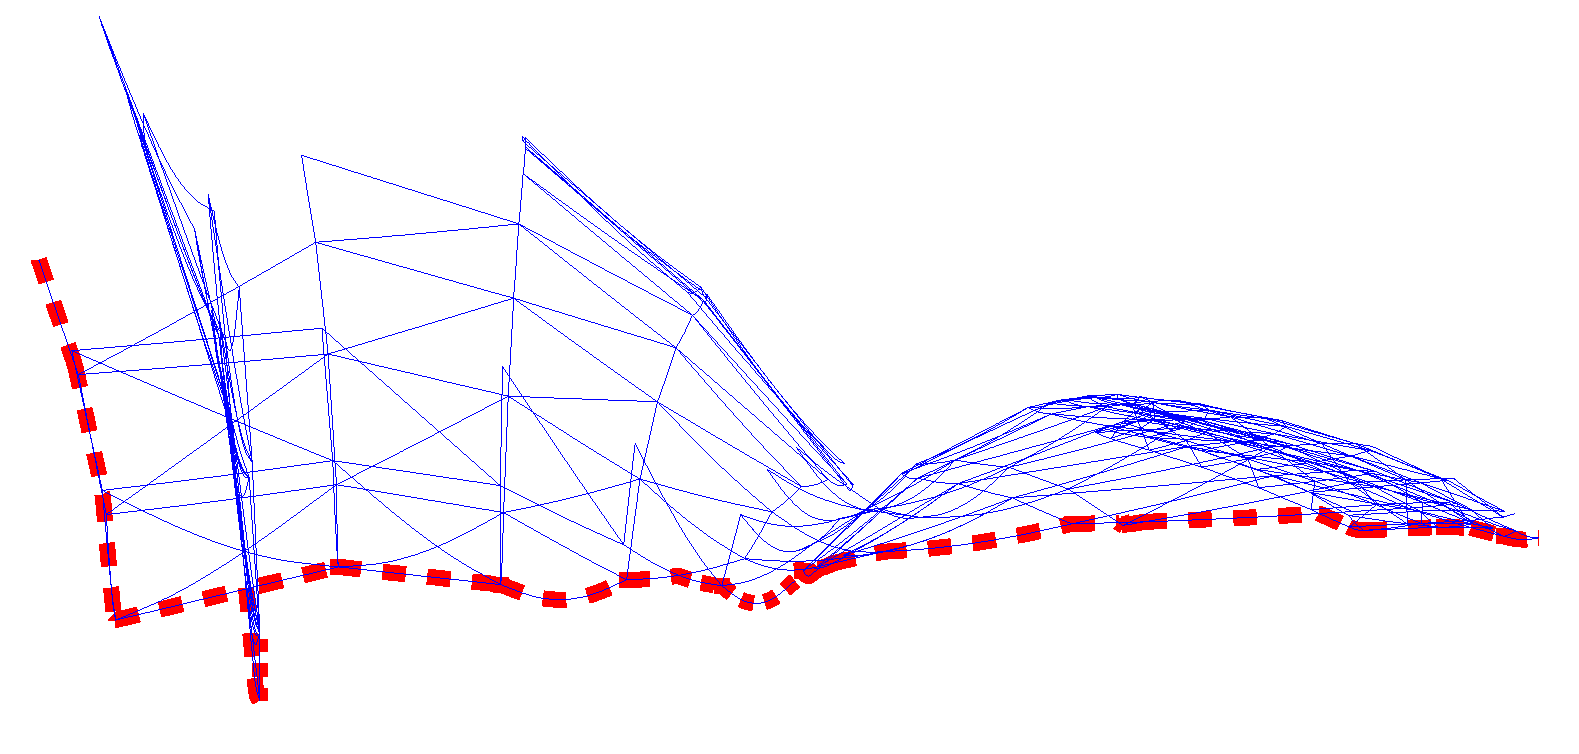
\includegraphics[width=5in]{Envelope_2/fig/lwrenv}
\end{ccTexOnly}
\label{fig:teaser}
\begin{ccHtmlOnly}
  <p><center>
    <img src="./fig/lwrenv.gif" border=0 alt="Lower Envelope">
  </center>
\end{ccHtmlOnly}
\caption{The lower envelope of a set of line segments and hyperbolic
arc.} 
\end{center}
\end{figure}

\section{Introduction}

A continuous curve $C$ in ${\mathbb R}^2$ is called {\em $x$-monotone}, if
every vertical line intersects it at a single point at most. For
example, the circle $x^2 + y^2 = 1$ is {\em not} $xy$-monotone as the
vertical line $x = 0$ intersects it at $(0, -1)$ and at $(0, 1)$;
however, it is possible to split the circle into an upper part and a
lower part, such that both of these parts are $x$-monotone.
We consider vertical segments as {\em weakly} $x$-monotone, to properly
handle inputs that contain such vertical curves.

An $x$-monotone curve can be represented as a univariate function
$y = C(x)$, defined over some continuous range $R_C \subseteq {\mathbb R}$.
Given a set ${\cal C} = \{ C_1, C_2, \ldots, C_n \}$ of $x$-monotone
curves, their {\em lower envelope} is defined as the point-wise minimum of
all curves. Namely, the lower envelope of the set ${\cal C}$ can be
defined as the following function:
\begin{eqnarray*}
{\cal L}_{{\cal C}} (x) = \min_{1 \leq k \leq n}{\overline{C}_k (x)} \ ,
\end{eqnarray*}
where we define $\overline{C}_k(x) = C_k(x)$ for $x \in R_{C_k}$,
and $\overline{C}_k(x) = \infty$ otherwise.

Similarly, the {\em upper envelope} of ${\cal C}$ is the point-wise maximum of
the $x$-monotone curves in the set:
\begin{eqnarray*}
{\cal U}_{{\cal C}} (x) = \max_{1 \leq k \leq n}{\underline{C}_k (x)} \ ,
\end{eqnarray*}
where in this case $\underline{C}_k(x) = -\infty$ for $x 
\not\in R_{C_k}$.

Given a set of $x$-monotone curves ${\cal C}$, the {\em minimization
diagram} of ${\cal C}$ is a subdivision of the $x$-axis into cells,
such that the identity of the curves that induce the lower envelope
over a specific cell of the subdivision (an edge or a vertex) is the
same. In non-degenerate situations, an edge --- which represents a
continuous interval on the $x$-axis --- is induced by a single
curve (or by no curves at all, if there are no $x$-monotone curves
defined over the interval), and a vertex is induced by a single curve
and corresponds to one of its endpoints, or by two curves and
corresponds to their intersection point.
The {\em maximization diagram} is symmetrically defined for upper envelopes.
In the rest of this chapter, we refer to both these diagrams as
{\em envelope diagrams}.

Lower and upper envelopes can be efficiently computed using a
divide-and-conquer approach. First, note that the envelope diagram for
a single $x$-monotone curve $C_k$ is trivial to compute: we project
the boundary of its range of definition $R_{C_k}$ onto the $x$-axis
and label the features it induces accordingly. Given a set
${\cal D}$ of (non necessarily $x$-monotone) curves in ${\mathbb R}^2$,
we subdivide each curve into a finite number of weakly $x$-monotone 
curves, and obtain the set ${\cal C}$. Then, we split the set into two
disjoint subsets ${\cal C}_1$ and ${\cal C}_2$, and we compute their envelope
diagrams recursively. Finally, we merge the diagrams in linear time by
traversing both diagrams in parallel.

\section{The Envelope Diagram\label{env2_sec:env_diag}}
%=============================

The package basically contains two sets of free functions:
\ccc{lower_envelope_x_monotone_2 (begin, end, diag)} (similarly
 \ccc{upper_envelope_x_monotone_2()}) construct the envelope diagram
for a given range of $x$-monotone curves, while 
\ccc{lower_envelope_2 (begin, end, diag)} (similarly
\ccc{upper_envelope_2()}) construct the envelope diagram for a
range of {\em arbitrary} (not necessarily $x$-monotone) curves.
In this section we explain more on the structure of the envelope
diagram these functions output.

\begin{figure}[t]
\begin{ccTexOnly}
  \begin{center}
    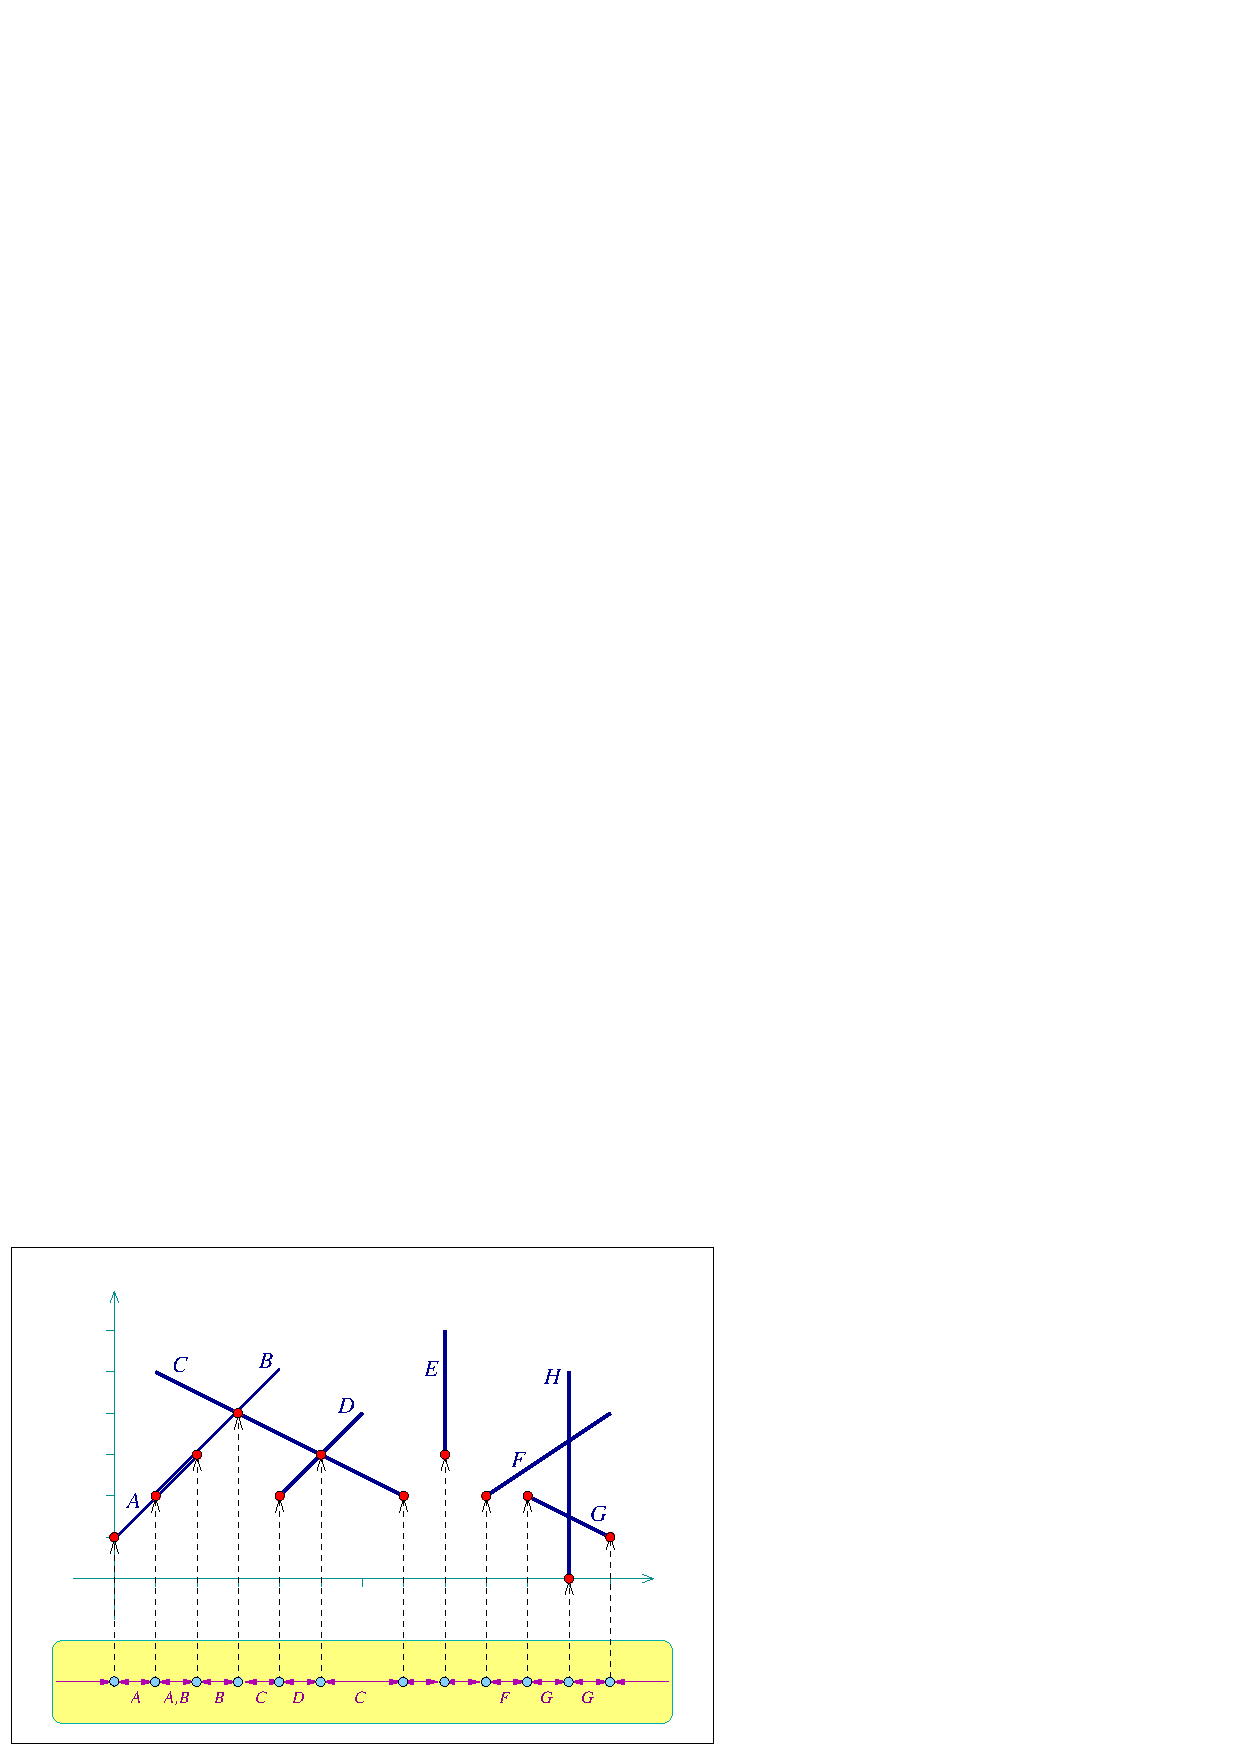
\includegraphics[width=5in]{Envelope_2/fig/min_diag}
  \end{center}
\end{ccTexOnly}
\begin{ccHtmlOnly}
  <p><center>
  <img src="./fig/min_diag.gif" border=0 alt="The minimization diagram">
  </center>
\end{ccHtmlOnly}
\caption{The lower envelope of eight line segments, labeled
$A, \ldots, H$\,, as constructed in \ccc{ex_envelope_segments.cpp}.
The minimization diagram is shown at the bottom, where
each diagram vertex points to the point associated with it, and the
labels of the segment that induce a diagram edge are displayed below
this edge. Note that there exists one edge that represents an overlap
(i.e., there are two segments that induce it), and there are also a 
few edges that represent empty intervals.\label{env2_fig:min_diag}}
\end{figure}

A minimization diagram or a maximization diagram is represented by
a model of the concept \ccc{EnvelopeDiagram_1}. This concept defines
the structure of the subdivision of the $x$-axis into $0$-dimensional
cells called {\em vertices}, and $1$-dimensional cells called {\em edges}.
The important property of this subdivision is that the identity of
the curves that induce the lower envelope (or the upper envelope)
over each cell is fixed.

Figure~\ref{env2_fig:min_diag} shows the lower envelope of a set of
eight line segments, and sketches the structure of their minimization
diagram. Each diagram vertex $v$ is associated with a point $p_v$ on
the envelope, which corresponds to either a curve endpoint
or to an intersection point of two (or more) curves. The vertex is
therefore associated with a set of $x$-monotone curves that induce the
envelope over $p_v$. Each vertex is incident to two edges, one lying
to its left and the other to its right.

An edge in the envelope diagram represents a continuous portion of the
$x$-axis, and is associated with a set of $x$-monotone curves that
induce the envelope over this interval. Note that this set may be
empty if no $x$-monotone curves are defined over this interval. In
degenerate situations where curves overlap, there may be more than
a single curve that induces the envelope over the interval the edge
represents. An envelop diagram of a set of curves either consists of
a single unbounded edge (in case the curve set is empty or if the
envelope contains a single unbounded curve that is below or above
all other curves), or at least one vertex and two unbounded edges,
while each additional vertex comes along with an additional edge. It
is possible to directly access the {\em leftmost} edge, representing
the unbounded interval that starts at $-\infty$, and the {\em rightmost}
edge, representing the unbounded interval that ends at $\infty$.
(In the example depicted in Figure~\ref{env2_fig:min_diag} we have
only bounded curves, so the leftmost and rightmost edges represent
empty intervals. This is not the case when we deal, for example, with
envelopes of sets of lines.)

Any model of the \ccRefName\ concept must define a geometric
traits class, which in turn defines the \ccc{Point_2} and 
\ccc{X_monotone_curve_2} types defined with the diagram features.
The geometric traits class must be a model of the 
\ccc{ArrangementXMonotoneTraits_2} concept in case we construct
envelopes of $x$-monotone curves. If we are interested in handling
arbitrary (not necessarily $x$-monotone) curves, the traits class
must be a model of the \ccc{ArrangementTraits_2} concept. This
concepts refined the \ccc{ArrangementXMonotoneTraits_2} concept;
a traits class that models this concepts must also defines a
\ccc{Curve_2} type, representing an arbitrary planar curve, and
provide a functor for subdividing such curves into $x$-monotone
subcurves.

\section{Examples}
%=================

\subsection{Example for Envelope of Line Segments}

The following example demonstrates how to compute and traverse the
minimization diagram of line segments, as illustrated in
Figure~\ref{env2_fig:min_diag}. We use the curve-data traits
instantiated by the \ccc{Arr_segment_traits_2} class, in order to
attach a label (a \ccc{char} in this case) to each input segment.
We use these labels when we print the minimization diagram:

\ccIncludeExampleCode{Envelope_2/ex_envelope_segments.cpp}

\subsection{Example for Computing the Convex Hull with Envelopes}

The next example computes the convex hull of a set of input points
by constructing envelopes of unbounded curves, in our case lines
that are dual to the input points. Here use the
\ccc{Arr_linear_traits_2} class to compute the lower envelope of the
set of dual lines. We read a set of points ${\cal P} = p_1, \ldots, p_n$
from an input file, and construct the corresponding dual lines
${\cal P}^{*} = p^{*}_1, \ldots, p^{*}_n$, where the line $p^{*}$ dual
to a point $p = (p_x, p_y)$ is given by $y = p_x x - p_y$. We then
compute the convex hull of the point-set ${\cal P}$, using the fact that
the lines that form the lower envelope of ${\cal P}^{*}$ are dual to the
points along the {\em upper} part of ${\cal P}$'s convex hull, and the
lines that form the upper envelope of ${\cal P}^{*}$ are dual to the
points along the {\em lower} part of the convex hull; see,
e.g.,~\cite[Section~11.4]{bkos-cgaa-00} for more details.
Note that the leftmost edge of the minimization diagram is associated
with the same line as the rightmost edge of the maximization diagram,
and vice-verse. We can therefore skip the rightmost edges of both
diagrams:

\ccIncludeExampleCode{Envelope_2/ex_convex_hull.cpp}

\begin{figure}[t]
\begin{ccTexOnly}
  \begin{center}
    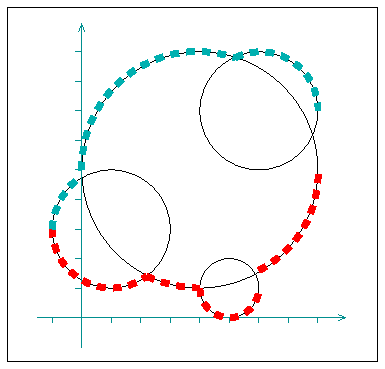
\includegraphics{Envelope_2/fig/ex_circle}
  \end{center}
\end{ccTexOnly}
\begin{ccHtmlOnly}
  <p><center>
  <img src="./fig/ex_circle.gif" border=0 alt="Envelopes of circles">
  </center>
\end{ccHtmlOnly}
\caption{A set of four circles, as constructed in
\ccc{ex_envelope_circles.cpp}. The lower envelope and the upper
envelope are shown using thick dashed lines of different colors
respectively.\label{env2_fig:ex_circ}}
\end{figure}

\subsection{Example for Envelope of Non-Linear Curves}

We conclude by an example of envelopes of non-linear curves. 
We use the \ccc{Arr_circle_segment_traits_2} class to construct the
lower and the upper envelopes of a set of four circles, as depicted
in Figure~\ref{env2_fig:ex_circ}. Note that unlike the two previous
examples, here our curves are not $x$-monotone, so we use the functions
that compute envelopes of arbitrary curves:

\ccIncludeExampleCode{Envelope_2/ex_envelope_circles.cpp}
